\documentclass[11pt]{article}
\usepackage{geometry}                % See geometry.pdf to learn the layout options. There are lots.
\geometry{letterpaper}                   % ... or a4paper or a5paper or ... 
%\geometry{landscape}                % Activate for for rotated page geometry
%\usepackage[parfill]{parskip}    % Activate to begin paragraphs with an empty line rather than an indent
\usepackage{graphicx}
\usepackage{amssymb,amsfonts,amsmath}
\usepackage{epstopdf}
\DeclareGraphicsRule{.tif}{png}{.png}{`convert #1 `dirname #1`/`basename #1 .tif`.png}

\title{Poisson model with adjusted confidence intervals for overdispersed plankton counts}

\begin{document}
\maketitle
\section{choice of model}

Goal: we'd like a way of constructing a seasonal climatology of plankton concentration, but without worrying about how interannual variation may distort or obscure the underlying seasonal pattern (i.e. cell abundance for a given season is really high one year, but zero the next year, such that averaging really doesn't do a good job). This can be accomplished using a model that accounts for both a season effect and year affect. Normally, the Poisson distribution does a job of representing count data. However, plankton counts at MVCO tend to be overdispersed relative to the Poisson distribution. 

Andy had mentioned that there are a few options to account for overdispersion (which may or may not simultaneously account for the over-occurrence of zeros). One option is a negative binomial model, of which the Poission distribution is a special case. This model would incorporate a seasonal and yearly effect, but also an overdispersion estimate for each season and year. While straightforward to design, it results in a large number of parameters that need to be estimated simultaneously, for example 26 seasons + 10year effects + $10 \cdot 26$ overdispersion effects. There could be work arounds to fitting $\sim$ 300 parameters, but these would involve assumptions of some type of pattern to the overdispersion (i.e., constant, seasonal or scales with plankton abundance), which we could not find much evidence for in the data. 

Another concern would be the robustness of the estimate for each overdispersion parameter. Some season/year combinations have very few observations, making one skeptical of any fit that solely relies on a few observations. In lieu of this approach, Andy recommended that we simply fit a Poisson model that incorporates a seasonal and year affect, and account for the overdispersion with corrected confidence intervals. As the Poisson model can account for observations of zero, this approach indirectly handles these observations. Below describes this model and subsequent confidence interval inflation as well as the matlab scripts for the fitting procedure.

\section{the count model}

We first organize our data by year (denoted by $i$) and by two-week `seasons' (denoted by $j$). For a given plankton, let $y_{ijk}$ be replicate count $k$ in year $i$ and season $j$. Likewise, we have corresponding volumes for each replicate count, denoted by $v_{ijk}$. Let $Y_{ij}$ be the sum of all counts:
$Y_{ij}=\sum_ky_{ijk} $ and likewise, $V_{ij}=\sum_k v_{ijk}$ be the sum of all volumes over the replicates in a season and year. Let's then assume that the counts vary according to a Poisson model:
\[
Y_{ij} \sim \text{Poisson}(\mu_{ij} \cdot V_{ij}),
\]
where $\mu_{ij}$ is the density of cells per volume for season $j$ and year $i$. We can then parameterize this density to have both a seasonal component and a yearly component:
\[
\mu_{ij}=\exp(\beta_i + \gamma_j).
\]
The exponential is there to ensure that the mean is positive, as required for the Poisson distribution. For the 2007-2016 data, this will give us 10 yearly effects ($\beta$'s) and 26 seasonal effects ($\gamma$'s). To fit this model with the data, we use a maximum likelihood approach. The Poisson probability mass function (pmf) is:
\[
\text{P(m events in an interval)} =  \frac{\lambda^me^{-\lambda}}{m!}
\]
where $\lambda$ is the mean number of events/counts in an interval and $m$ is the number of events/counts for that interval. In our case, for a given season/year, the pmf becomes:
\[
P(Y_{ij}) =  \frac{(\mu_{ij}\cdot V_{ij})^{Y_{ij}}    e^{-(\mu_{ij} \cdot V_{ij})}   } {Y_{ij}!} =  \frac{(\exp(\beta_i + \gamma_j)\cdot V_{ij})^{Y_{ij}}    \exp(-(\exp(\beta_i + \gamma_j) \cdot V_{ij}))   } {Y_{ij}!}
\]

We then calculate the log likelihood function as:
\begin{align}
\notag
L(\mathbf{\beta},\mathbf{\gamma}) =& \prod_{i=1}^{10} \prod_{j=1}^{26} P(Y_{ij}) \\\notag
\log L(\mathbf{\beta},\mathbf{\gamma}) =& \sum_{i=1}^{10} \sum_{j=1}^{26} \log P(Y_{ij}) \\\notag
\log L(\mathbf{\beta},\mathbf{\gamma}) =& \sum_{i=1}^{10} \sum_{j=1}^{26} \left[ Y_{ij} ( \beta_i + \gamma_j + \log V_{ij}) - \exp(\beta_i + \gamma_j) V_{ij} \right]
\end{align}

We search over 36 parameters to find the values that maximize this function, given the data. However, there is an additional constraint that must be imposed to be able to find a distinct solution. Because the mean density is an additive combination between two sets of parameters, it is the sum or difference between them that will determine the likelihood value. Because of this, you could have several different sets of parameters that would equally generate the same "difference". For example, $\beta_1 = 2$ and $\gamma_1= -1$ gives $\mu_{1,1} = \exp(1)$, but so does ($\beta_1 = 4$, $\gamma_1= -3$) or ($\beta_1 = -4$, $\gamma_1= 5$). To avoid this problem, we set an `identifiability' constraint. This can take a few forms, such as $\beta_1 = - \sum_{i=2}^{10}\beta_i$, or $\beta_1 =0$. The maximum likelihood estimates of parameters are therefore interpreted relative to this constriant (i.e. parameters are relative to a mean year effect or relative to the first year). We will set $\beta_1 = - \sum_{i=2}^{10}\beta_i$ as this is a bit easier to interpret (more on that later).

With maximum likelihood estimators in hand, we can then construct confidence intervals for each parameter. We do this with use of the standard likelihood ratio test with profile log likelihoods for each parameter:
\[
2\left[ \log L(\hat{\beta},\hat{\gamma}) - \log_{\text{prof}}(\beta_i \text{ or } \gamma_j) \right] \sim \chi^2_1,
\]

\noindent where $(\hat{\beta},\hat{\gamma})$ are the maximum likelihood estimates of the parameters, $\log_{\text{prof}}$ refers to the profile log likelihood of a given parameter ($\beta_i \text{ or } \gamma_j$; constructed by holding the parameter at a certain value and resolving for the rest of the parameters that maximize the likelihood function for this value), and $\chi^2_1$ is the chi-squared distribution with 1 degree of freedom. We then search over the range of a given parameter to find the values that satisfy this inequality at significance level $\alpha=0.05$ (see Figure 1). Note that profile likelihoods are also constructed with the identifiability constraint of $\beta_1 =0$.

\begin{figure}[h]
\centering
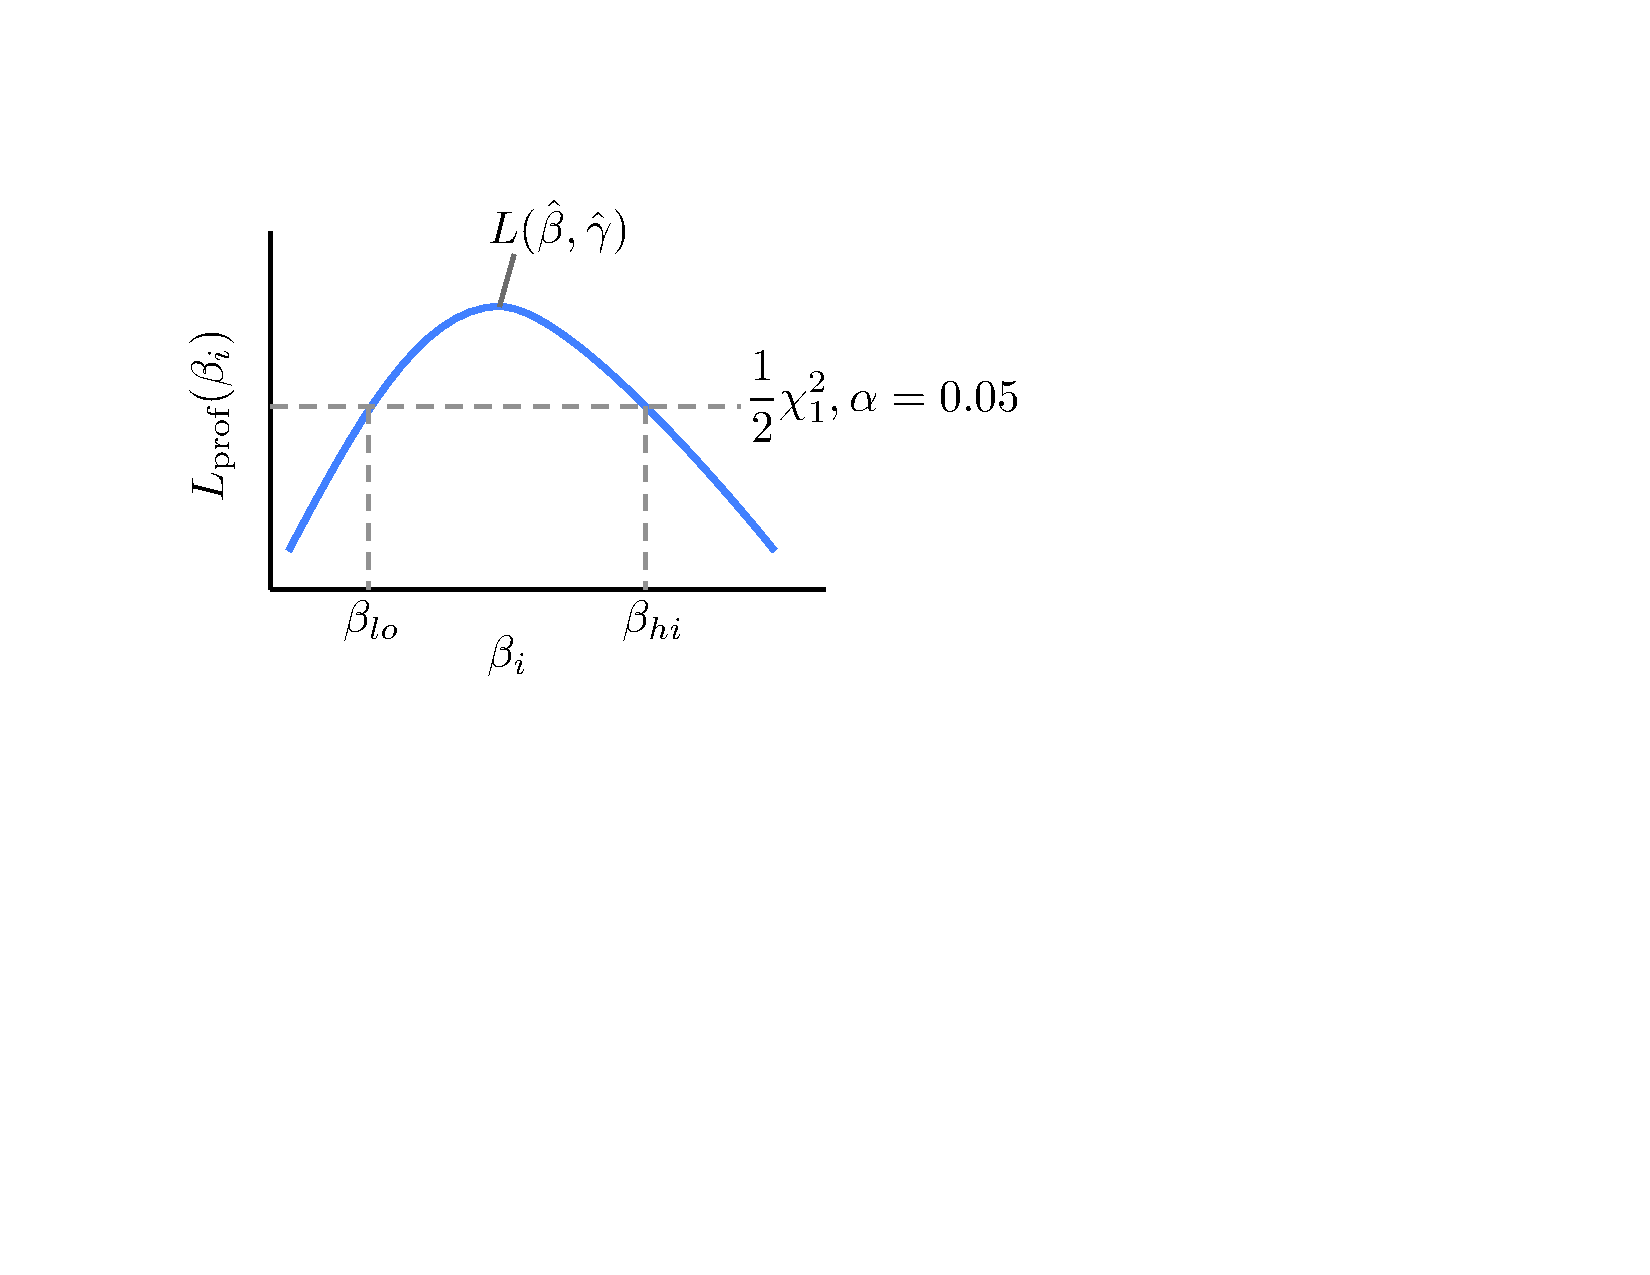
\includegraphics[width=0.6\textwidth]{logL_figure.pdf}
\caption{Schematic of profile likelihood and relationship to confidence intervals.}
\end{figure}

\pagebreak
If the counts are over-dispersed, we inflate the confidence intervals with a calculated metric for overdispersion. To do this, we first form the Pearson statistic (also denoted by $\chi^2$):
\[
 \chi^2 = \sum_{i=1}^{I} \sum_{j=1}^{J} \frac{(y_{ij} - \hat{y}_{ij})^2}{\hat{y}_{ij}},
\]

\noindent where $\hat{y}_{ij} = \exp(\hat{\beta}_i + \hat{\gamma}_j) V_{ij}$, and $I$ is the total number of years and $J$ is the total number of seasons for which there is at least one non-zero count. We leave out seasons or years that have all zero counts as these will not contribute to calculating an overdispersion metric (and we cannot actually evaluate the Pearson statistic in these cases (the denominator will be 0)). When then define a quantity $c$ as a multiplier for the $\chi^2_1$ $\alpha=0.05$ significance value:
\[
c = \max \left[1, \frac{\chi^2}{(I\cdot J - (I + J))}\right]
\]
The corrected 0.95 confidence interval for say $\beta_1$, is then given by the values of $\beta_1$ that satisfy:
\[
2 \left[ \log L (\hat{\beta},\hat{\gamma}) - \log L_{\text{prof}}(\beta_1)) \right] < \chi^2_1 \cdot c,
\]
where the $\log L_{\text{prof}}$ is the profile log likelihood based on the Poisson assumption.  Note that this approach gives the option of not having over dispersed data if the maximum value between 1 or $ \frac{\chi^2}{(I\cdot J - (I + J))}$ is indeed 1.For the data that has all zero counts for a given season or year, only an upper bound of the confidence interval can be found, where the lower bound will try to go to $-\infty$ (the seasonal or yearly parameter will numerically try to get the quantity $\exp(\beta_i + \gamma_j)$ as close to zero as possible to yield a mean density of 0, but as only $\lim_{x \to -\infty} \exp(x) =0$, a true lower bound does not exist). We also are not able to construct a confidence interval for $\beta_1$ as we have used this for our reference for other parameters.

 
\section{matlab scripts} 

The matlab scripts to fit this model and construct confidence intervals are listed below along with short descriptions. These are called from the main wrapper script, \textbf{opt\_max\_logL.m}, which in addition to the functions below, also sets up the data in expected format and generates some figures to compare data to fitted model. Nested lists indicate script dependencies.

%\begin{description}
%\item [opt\_max\_logL.m] overarching wrapper script from where other scripts are called
%\item [poisson\_logL.m] calculates a negative log likelihood value given a set of parameters and count data
%\item [poisson\_logL\_prof.m] script that returns a negative log likelihood value given a set of parameters and count data but for use in profile log likelihood evaluation.
%\end{description}

\begin{itemize}
\item maximum likelihood estimate of parameters:
\begin{description}
\item [poisson\_logL.m] function called by optimization routine; calculates a negative log likelihood value given a set of parameters and count data
\end{description}

\item confidence interval construction:
\begin{description}
\item [poisson\_est\_CIs.m] script that sets up root solver to find parameter values that satisfy likelihood ratio test inequality with inflated value based on overdispersion metric 
\begin{description}
\item [eval\_param\_for\_CIs.m] function called by root solver; with specified parameter value calculates a profile log likelihood by resolving for parameter values that minimize negative log likelihood
\begin{description}
\item [poisson\_logL\_prof.m] function called by optimization to find parameter values that minimize negative profile log likelihood
\end{description}
\end{description}
\end{description}
\end{itemize}


\section{interpretation of seasonal and year effects} 

One of the main goals of this approach is to be able to produce a seasonal climatology without the influence of interannual variation. If we fit with the model with an identifiability constraint of $\beta_1 = - \sum_{i=2}^{10}\beta_i$ (or another year of choice), a climatology is retrieved from the exponential of the fitted seasonal parameters ($\exp(\gamma_j)$).  Because the year parameters are fit such that their average is zero, the value of the fitted seasonal parameters are relative to a `zero' year affect, which is exactly what we would like for a climatology.  

With simulated data, for example, we see that the estimated year effects are equally distributed around zero (as required by the identifiability constraint) and shifted by some amount from the true year parameters used to simulated the data (shifted by the mean of the true year parameters). The seasonal parameters are also shifted by this amount, only in the opposite direction. With this identifiability constraint, no matter which year is `left out', the resulting seasonal and year parameter estimates are the same (which is not true in the case of an identifiability constraint of $\beta_i=0$).

\begin{figure}[h]
\centering
\includegraphics[width=0.7\textwidth]{simdata1.pdf}
\caption{True and estimated parameters of simulated data. A. Seasonal parameters. B. Year parameters.}
\end{figure}

\clearpage

We can write these relationships as follows:
\begin{align}
\beta_i &= \hat{\beta_i} - \bar{\beta}\label{eqn1} \\
\gamma_j &= \hat{\gamma_j} + \bar{\beta} \label{eqn2}
\end{align}

\noindent where $\beta_i$ and $\gamma_j$ are the true parameters, $\hat{\beta_i}$ and $\hat{\gamma_j}$ are the parameter estimates fitted with the identifiability constraint, and $\bar{\beta}$ is the mean of the true year parameters. These relationships also show that it is only the absolute distance between the year and seasonal parameters that matter:
\begin{align}
\beta_i + \gamma_j &= \hat{\beta_i} - \bar{\beta} + \hat{\gamma_j} + \bar{\beta} \\
\beta_i + \gamma_j &= \hat{\beta_i} + \hat{\gamma_j} \label{eqn4}
\end{align}


A plot of density of simulated data and the estimated density from maximum likelihood parameters (those in Figure 2) illustrates this concept:
 
 \begin{figure}[h]
\centering
\includegraphics[width=0.9\textwidth]{simdata2.pdf}
\caption{Density of simulated data (blue line) and estimated density from fitted parameters (orange squares).}
\end{figure}


\subsection{units}
 In the model formulation above, the parameters are linear in the log space, such that both $\beta_i$ and $\gamma_j$ should be in units of ln(cells mL$^{-1}$). This ends up being a rather tricky interpretation if the exponential is re-arranged:

\begin{align}
\mu_{ij} &= \exp(\beta_i +\gamma_j) = \exp( \log (\frac{\text{cells}}{\text{mL}}) + \log(\frac{\text{cells}}{\text{mL}}) \\
\mu_{ij} &= \exp(\beta_i)\exp(\gamma_j) = \exp(\log(\frac{\text{cells}}{\text{mL}}))\exp(\log(\frac{\text{cells}}{\text{mL}}) \\
\mu_{ij} &= \left( \frac{\text{cells}}{\text{mL}}\right)^{2} \text{  ???}
\end{align}

To avoid this we could present the model as such:
\[
\mu_{ij} = \alpha_i\exp(\gamma_j), \text{ where } \alpha_i > 0,
\]

\noindent where $\alpha_i$ is to be interpreted as a scale factor and is unitless. To ensure $\alpha_i$ is always positive, we could set $\alpha_i =\exp(\beta_i)$ and the construction and fitting is the same as described above. To avoid interpretation issues, we will go with this presentation.


%Doesn't really make much sense below....
%Alternatively, one could just simply do the addition before taking the exponential. However, the relationship in Eqn.~\ref{eqn4} can help with an alternative unit interpretation, where the units are attached to the fitted seasonal parameters and the year parameters are interpreted as `scale' factors. For simply an estimated seasonal climatology we have:
%

%\begin{align}
%\mu_{j} &= \exp(\hat{\gamma_j}) \\
%\mu_{ij} & = \exp\left(\gamma_j - \bar{\beta} \right) \\
%\mu_{ij} & = \exp(\gamma_j + \hat{\beta_i} - \beta_i) \\
%\mu_{ij} & = \frac{\exp(\hat{\beta_i})}{\exp(\bar{\beta})}\exp(\hat{\gamma_j} + \bar{\beta}) = \frac{\text{cells/mL}}{\text{cells/mL}} \left(\frac{\text{cells}}{\text{mL}}\right)
%\end{align}

\subsection{real data}

Here we apply the model to observed counts of \textit{Laboea strobila} at MVCO from 2007-2016. 

\begin{figure}[h]
\centering
\includegraphics[width=0.7\textwidth]{Laboea1.pdf}
\caption{A. Observed cell densities of \textit{Laboea strobila} from 2007-2016 (gray lines, aggregated density for each manually classified sample (total cells observed in two-week time window divided by total volume analyzed in same time window)), estimated seasonal density pattern from maximum likelihood estimates of seasonal parameters (($\exp(\hat{\gamma}_i)$), blue line) with 95\% confidence intervals (light blue lines), and mean cell density of season across all years (red line). B. Year multiplier effect for each year $(\exp(\beta_i))$, with confidence intervals.}
\end{figure}

For reference, the mean density (calculated by taking the average of densities for each time window across all years) is presented (red line). Note that this does not exactly match the expected seasonal densities from the model due to year affects being intrinsically incorporated into the calculation.

The observed cell density and estimated density (calculated from $\exp(\beta_i+\gamma_j)$) is shown in Figure 5. For this data, the default MATLAB solver tolerances did not always allow convergence to the global minimum. Setting the optimality tolerance (minimum gradient change) lower seemed to resolve this. It would good though to simply run the solver with each year left out (for the idenitifiability constraint) and check whether or not the maximum likelihood values are indeed the same (they should be). If there is a discrepancy, setting the start-point for the solver as the end solution for another year may  help. Parameters that truly tend towards zero also may not come back as the exact value (i.e -13, -14.5, -16 equate to simply a very small number when the exponential is taken). 


\begin{figure}[h]
\centering
\includegraphics[width=0.9\textwidth]{Laboea2.pdf}
\caption{Observed cell densities of \textit{Laboea strobila} from 2007-2016 (gray line) with estimated density from maximum likelihood estimates parameters (blue line).}
\end{figure}

The year affects, while a bulk multiplier, could be investigated with regard to relationships with environmental variables. 

\clearpage

\section{test for overdispersion}        

How did we find out that our counts were overdispersed in the first place? Andy provided two tests to investigate this: one a full significance test and the other metric based.\\

\noindent \textbf{Significance test:} According to Andy, under the Poisson assumption, the conditional distribution of the replicate counts within a season/year is multinomial, with the number of trials being the replicates $k$, and success probability $p$, where:
\[
p_k = \frac{v_k}{\sum_{k=1}^K v_k},
\]
depends on volume sampled for each replicate ($K$ is total number of replicates for one season/year). The Poisson assumption can be assessed by testing the null hypothesis that these probabilities are as given, or agree with the observed data. To do this, we use a standard Chi-squared goodness of fit test between the observed and expected. The test statistic is:

\[
\chi^2 = \sum_{k=1}^K \frac{(y_k-np_k)^2}{np_k},
\]

\noindent where n is the total counts of plankton across all replicates, $n= \sum_{k=1}^K y_k$. Under the null hypothesis, this metric has an approximate $\chi^2$ distribtuion with $K-1$ degrees of freedom. This approximation won't work well if a lot of the quantities $np_k$ are small. One could assess significance with a parametric bootstrap in that case.\\
                                               
\noindent \textbf{Less formal approach:} A less formal way to make an assessment of the Poisson assumption is based on the quantity:
\[
\frac{\chi^2}{(K-1)}
\]

\noindent If this quantity is systematically or much greater than 1, then the data is likely overdispersed. This is especially useful for getting a feel for how overdispersion varies over the timeseries, although Andy cautioned not to get too excited by a few peaks. The matlab script that performs these calculations is \textbf{test\_poisson\_overdisp.m}

\end{document}  